%--------------------------------------------
% section: Angle calculation
%--------------------------------------------

%--------------------------------------------
% Chapter: SENSOR FUSION OF INERTIAL MEASUREMENT UNIT
%--------------------------------------------
\chapter{Sensor fusion for Inertial Measurement Unit}
\label{sec:sensorFusion}

\section{Angle calculation}
\label{sec:angle}

\subsection{Calculation of the orientation angles}
\label{subsec:CalcAngle}
The Kalman filter and the Complementary filter both need angles as input. Those angles are calculated with the acceleration sensor and with the gyroscope. The gyroscope sensor is used as main input and is corrected by the acceleration/magnetic sensor. The reason why both are used is already described in the Sensor fusion chapter.\\
To achieve an angle from the gyroscope, the values from the sensor needs to be integrated. The following formulas show the integration part of the function of the gyroscope which runs on the Raspberry Pi. It is located in the folder 'sig/Orientientation/' in the file Orientation.c in the function 'm\_sigOri\_calcGyroAnglePerStep\_st()'. This function calculates the angle which since the last call is made.
\begin{align}
roll_{angle}&=roll_{rate}*deltaT\\
pitch_{angle}&=pitch_{rate}*deltaT\\
yaw_{angle}&=yaw_{rate}*deltaT
\end{align}
To make this code independent from any time step, it calculates locally the time difference 'deltaT' between the last call. To make this possible the 'gettimeofday' function is used. Because of that any jitter will not make a problem. Also the gyroscope sensor gets automatically offset corrected when the code is started.\\\\
To get an angle from the acceleration/magnetic sensor the following calculation is needed. It is located in the function 'm\_sigOri\_calcAccMagAngle\_st()' in the same file like mentioned before.\\
First the roll angle is calculated:
\begin{align}
roll_{angle\_rad}&=atan2\left(\frac{acc_{y\_axis}}{acc_{z\_axis}}\right)\\
		roll_{angle\_deg}&=-roll_{angle\_rad}*180/Pi
\end{align}

Then the pitch is calculated:
\begin{align}
pitch_{angle\_rad}&=atan\left(-\frac{acc_{x\_axis}}{acc_{y\_axis}*sin(roll_{angle\_rad})+acc_{z\_axis}*cos(roll_{angle\_rad})}\right)\\
pitch_{angle\_deg}&=-pitch_{angle\_rad}*180/Pi
\end{align}

Last step is the calculation of the yaw angle. The yaw angle can not be calculated by the acceleration sensor, only the magnetic sensor can be used for this. But the magnetic sensor can not directly be used. Additional a magnetic tilt compensation needs to be done. The following formulas show the calculation steps.\\
\begin{align}
divider=mag_{x\_axis}&*cos(pitch_{angle\_rad})+\\
mag_{y\_axis}&*sin(pitch_{angle\_rad})*sin(roll_{angle\_rad})+\\
mag_{z\_axis}&*sin(pitch_{angle\_rad})*cos(roll_{angle\_rad})
\end{align}
\begin{align}		
yaw_{angle\_rad}&=atan2\left(\frac{mag_{z\_axis}*sin(roll_{angle\_rad})-mag_{y\_axis}*cos(roll_{angle\_rad})}{divider}\right)\\
yaw_{angle\_deg}&=yaw_{angle\_rad}*180/Pi
\end{align}
With this, the implementation of the fusion filter were done and proved. First the results seem to be correct like can be seen in figure \ref{fig:initial_angle}.

\begin{figure}[H]
	\centering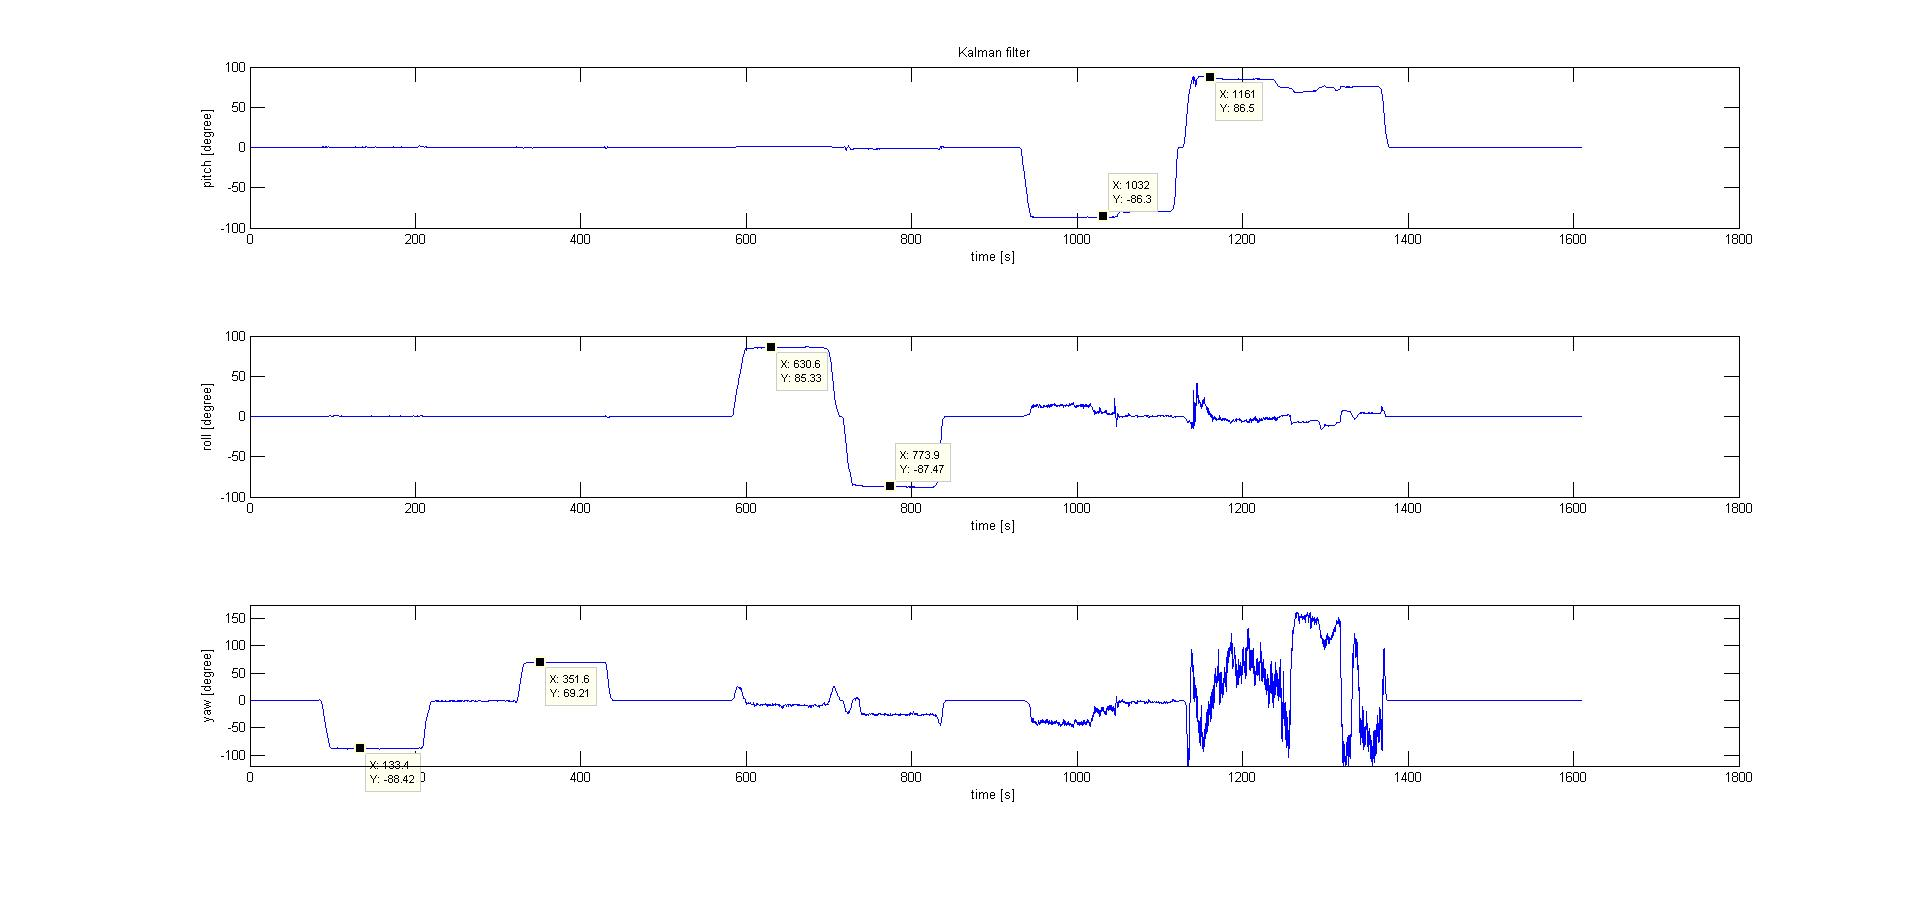
\includegraphics[width=1.0\textwidth]{fig/Res_Kal_Comp/initial_Kalman}
	\caption{First result Kalman filter}
	\label{fig:initial_angle}
\end{figure}
\subsection{Magnetic sensor test}
\label{subsec:MagSensTest}
As can be seen there is a problem with the yaw angle when a pitch angle is applied. This is no solution which can be used in the Quadrocopter. So additional tests are made. After some time the problem was detected. Because just the yaw angle makes some problem, the main observation layed on the magnetic sensor. Figure \ref{fig:field_weak} shows the measured magnetic field.
\begin{figure}[H]
	\centering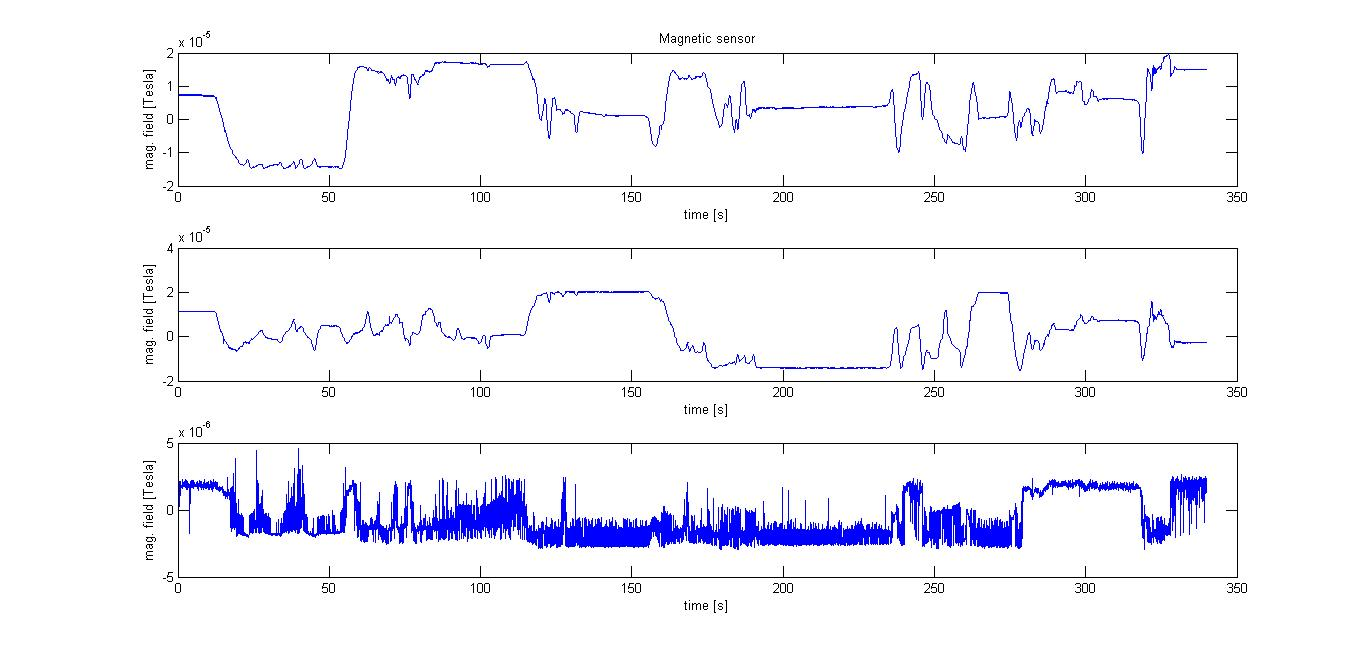
\includegraphics[width=1.0\textwidth]{fig/Res_Kal_Comp/field_weak}
	\caption{Weak magnetic field strength}
	\label{fig:field_weak}
\end{figure}
The problem can directly be seen. The measured field strength should be nearly the same on all axis. The field strength on the x-axis and y-axis is the same. The z-axis delivers only just one tenth of the normal value. Because of that the noise on the sensor is in the same height like the signal and therefore acquiring not possible. First the position of the mounted IMU is disputed.
After changing the following sensor values of the magnetic sensor can be achieved.
\begin{figure}[H]
	\centering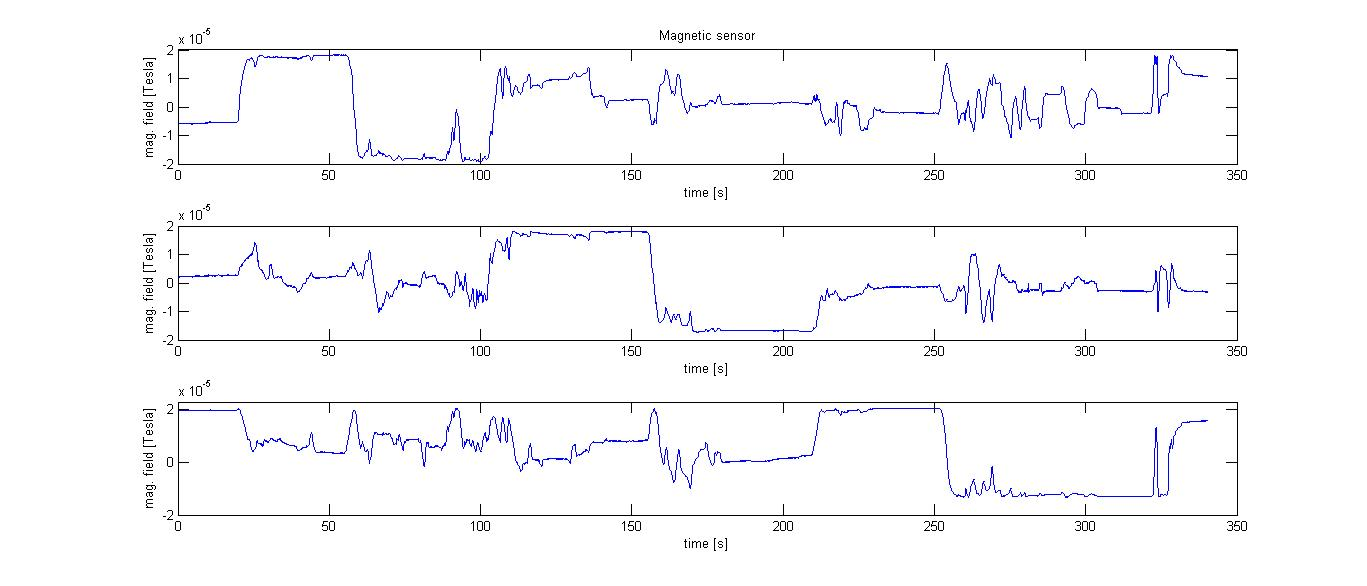
\includegraphics[width=1.0\textwidth]{fig/Res_Kal_Comp/field_strong}
	\caption{Strong magnetic field strength}
	\label{fig:field_strong}
\end{figure}
By comparing the measurement of the initial positioning of the IMU with the new one, the strength on the z-axis is significantly higher. Also the strength on the three axis are nearly the same. So for further usage the new position is used. 

\subsection{Improvement magnetic sensor}
\label{subsec:ImpMagSens}
The figures \ref{fig:pos_neu1} and \ref{fig:pos_neu2} shows the comparison of the mounting.
\begin{figure}[H]
	\centering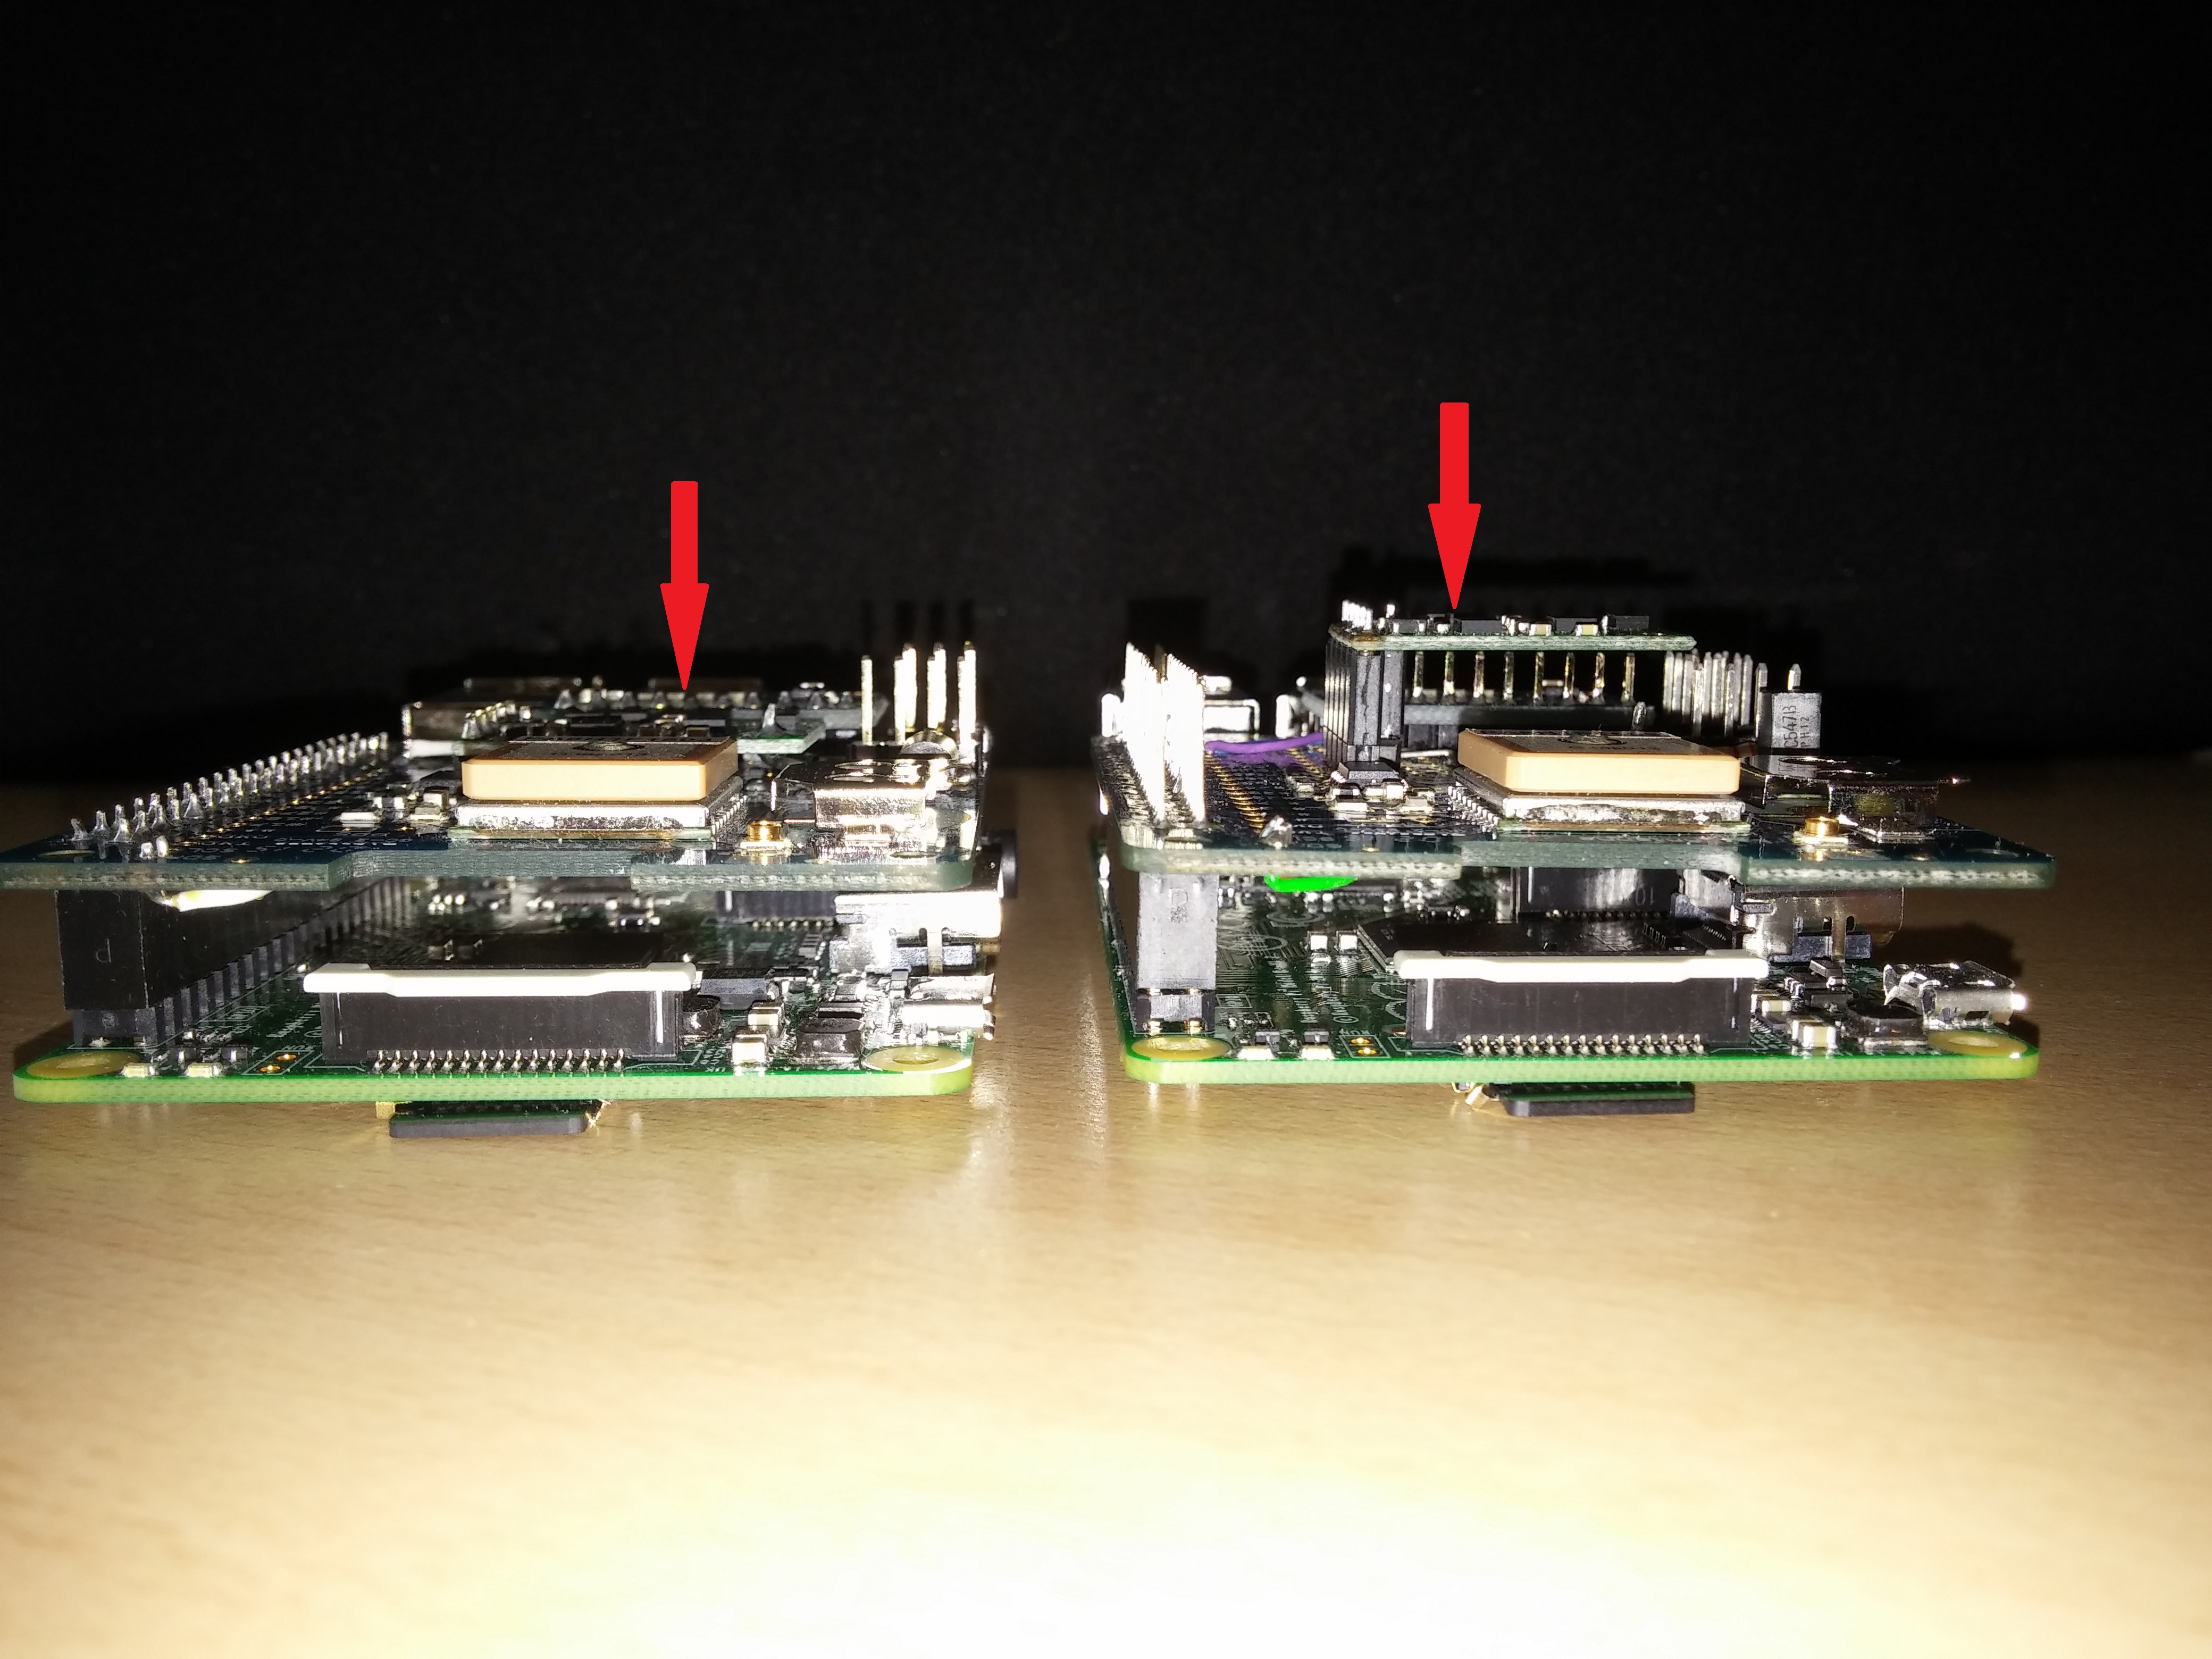
\includegraphics[width=0.6\textwidth]{fig/Res_Kal_Comp/pos_neu1}
	\caption{New positioning of IMU 1}
	\label{fig:pos_neu1}
\end{figure}
\begin{figure}[H]
	\centering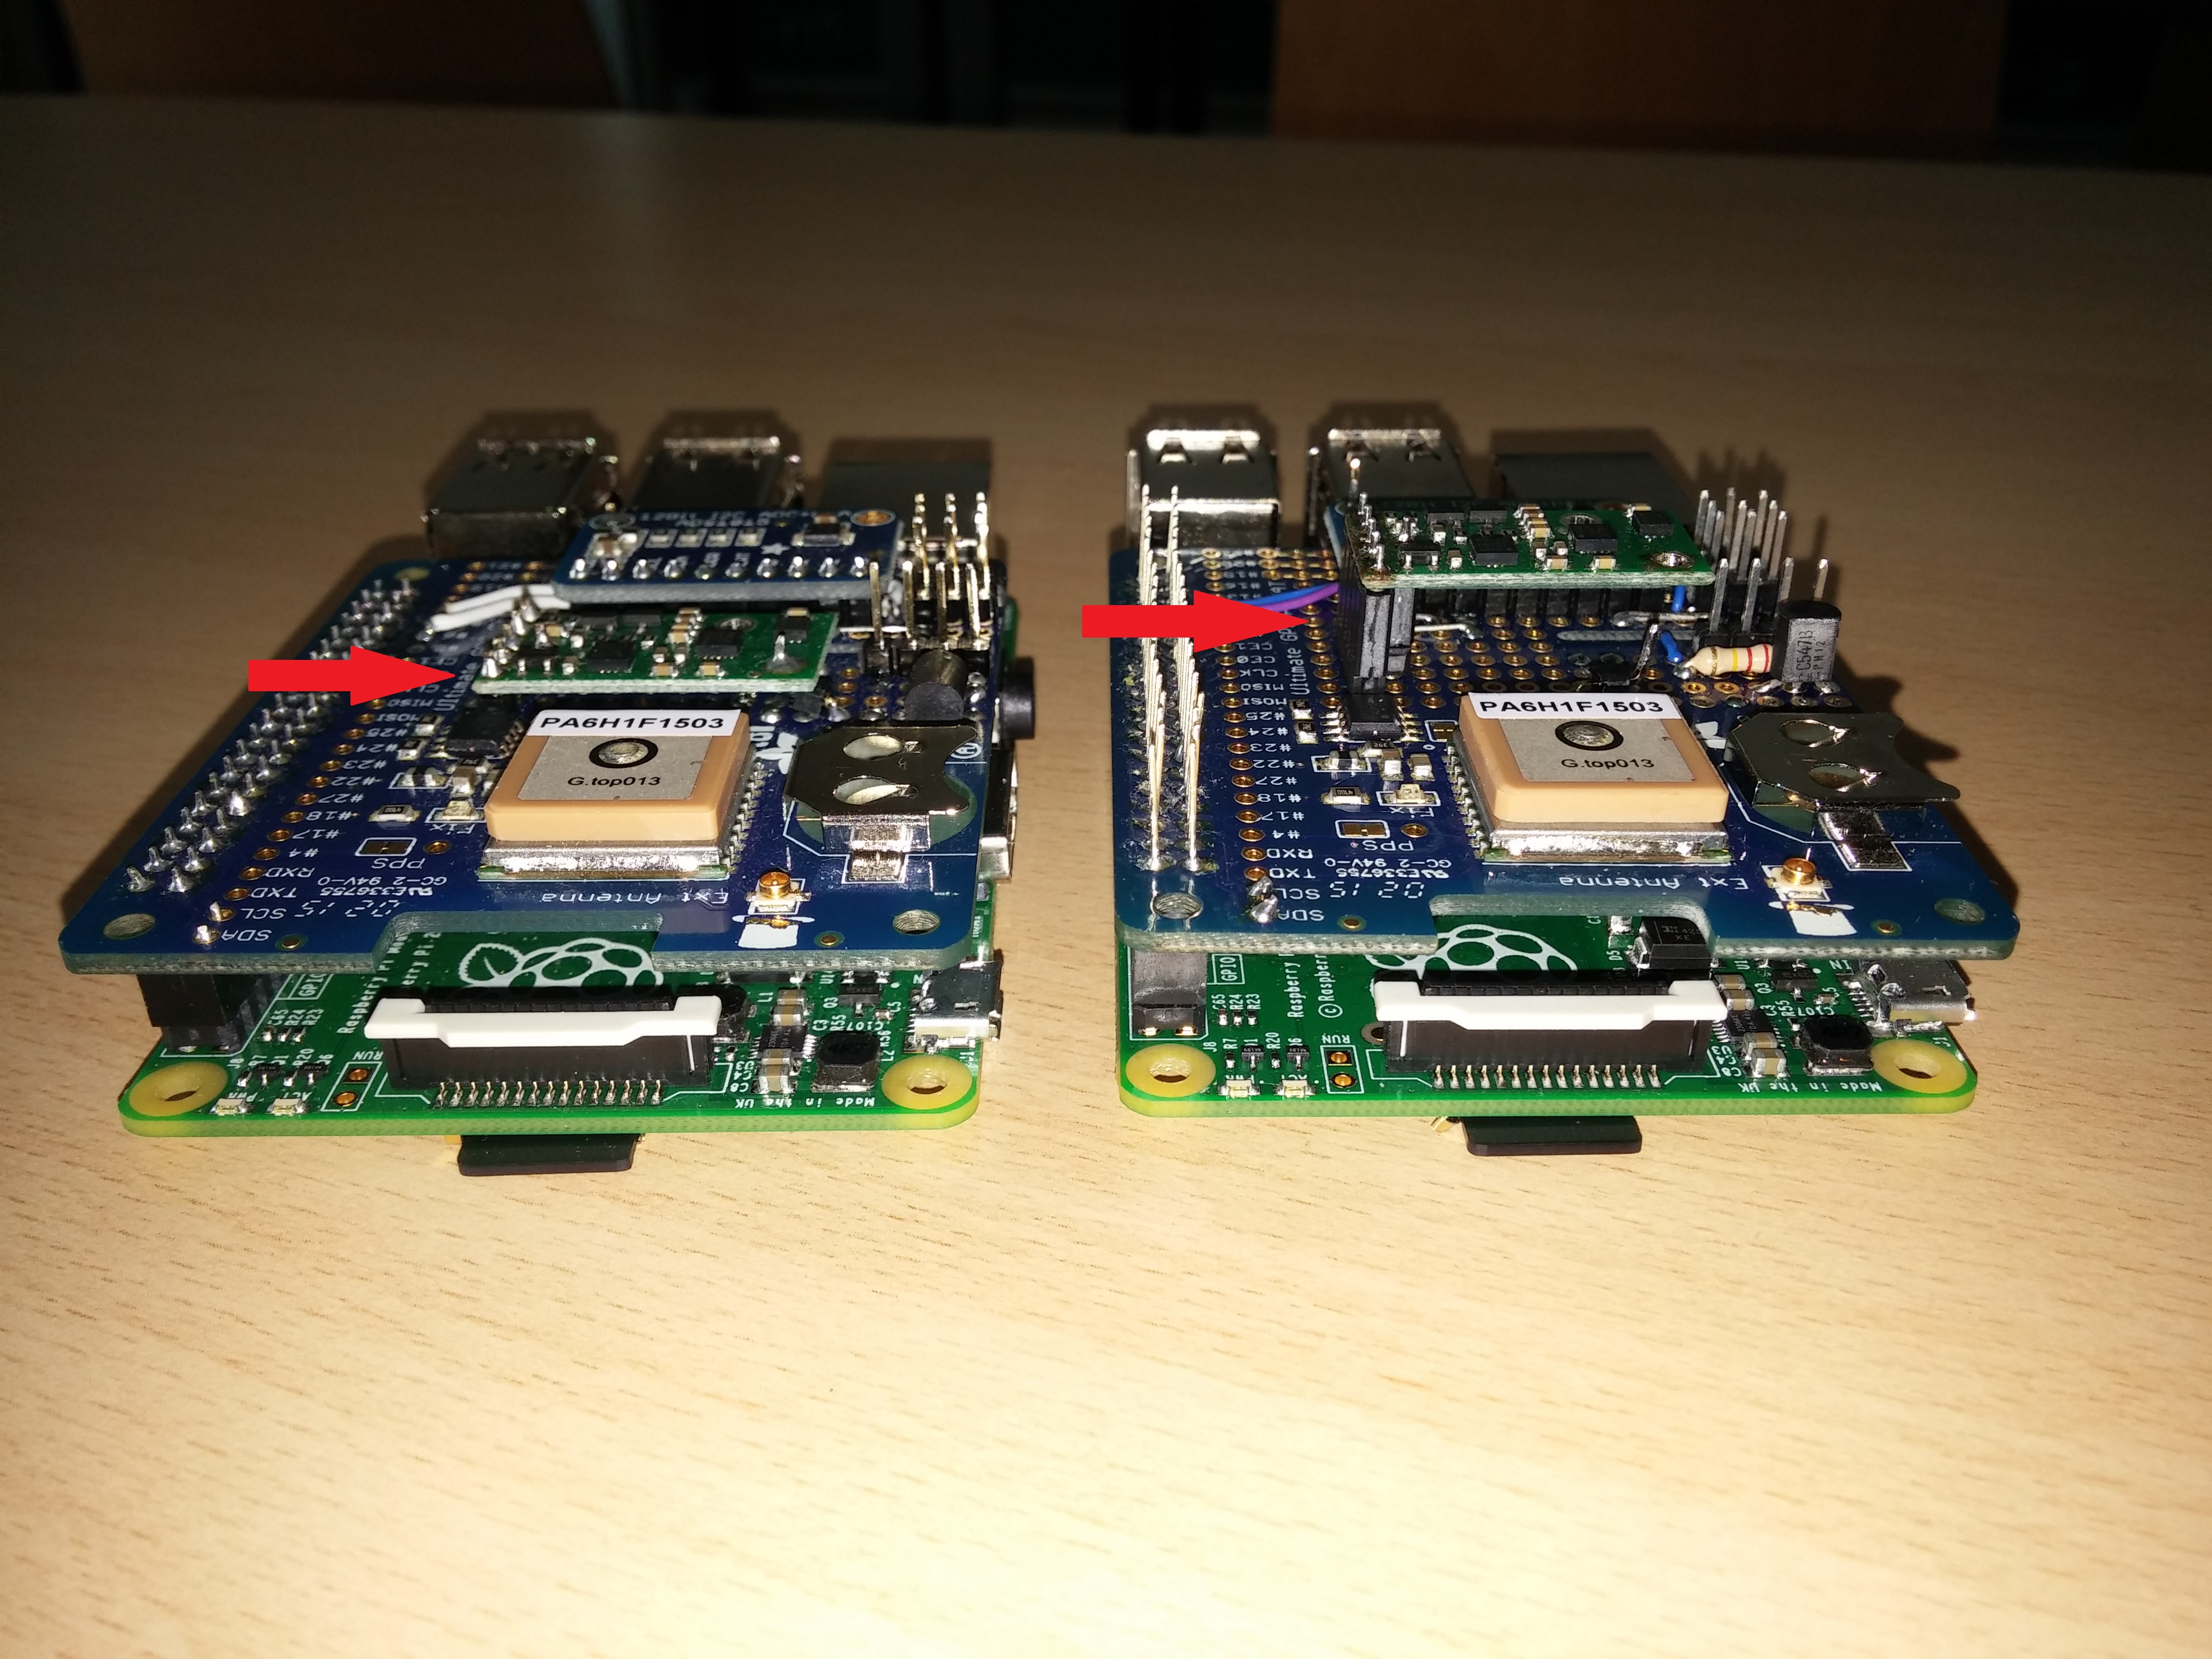
\includegraphics[width=0.6\textwidth]{fig/Res_Kal_Comp/pos_neu2}
	\caption{New positioning of IMU 2}
	\label{fig:pos_neu2}
\end{figure}
The left PCB shows the old position and the right the new position. As can be seen just the height of the mounted IMU needs to be changed. Due to the tests a distance of approximately 1cm seems to be enough. So the wiring can be kept as it is.\\
Additionally to reduce the really high influences of near metallic parts, a hard magnetic offset compensation needs to be done. Also a scaling is done. The following calculations which run in the function 'm\_sigOri\_calcAccMagAngle\_st()' are done within every step.
\begin{align}
mag_{x\_axis}=(mag_{x\_axis}-logged_{min\_x})/(logged_{max\_x}-logged_{min\_x})*2-1\\
mag_{y\_axis}=(mag_{y\_axis}-logged_{min\_y})/(logged_{min\_y}-logged_{min\_y})*2-1\\
mag_{z\_axis}=(mag_{z\_axis}-logged_{min\_z})/(logged_{min\_z}-logged_{min\_z})*2-1
\end{align}
To achieve the full range, maximum and minimum value of all three magnetic sensors the scope of Matlab can be used. First the data transmission between Matlab and the Raspberry Pi needs to be started. Then the scopes of the magnetic sensor should be opened. Now the Raspberry Pi should be rotated by parallel trying to find the maximum and minimum with the opened scopes. The m-file which is mentioned before creates directly the header-file for the code. The improved results due to the changes which are made here can be seen in the second output of the Kalman filter and complementary filter in figure \ref{fig:final_Comp} and \ref{fig:final_Kalman}.


%--------------------------------------------
% section: Complementary Filter result 
%--------------------------------------------

\section{Complementary-Filter}
\label{sec:ComplementaryFilterResult}

As written in the chapter about the sensor fusion for the complementary filter a filter time needs to be chosen. This constant is used for the lowpass filter for the acceleration/magnetic sensor and for the highpass filter of the gyroscope. \\\\
The complementary filter uses the following calculation:
\begin{align}
angle=alpha*(angle+integrated\_Gyro)+(1-alpha)*Acc\_Mag\_angle
\label{equ:Comp1}
\end{align}

As an initial guess for the first try the complementary filter uses the filter constant of 0.995. The sampling period of the sensors is 800 Hz. Usage of the filter constant of 0.995 and the sampling period of 800 Hz leads to a cut off frequency of 4 Hz. 
\begin{align}
alpha&=\frac{time\_constant}{time\_constant+sample\_period}
\label{equ:Comp2a}
\end{align}
\begin{align}
alpha&=0.995\\
sample\_period&=\frac{1}{800 Hz}=0.00125sec\\
\label{equ:Comp2b}
\end{align}
This leads to:
\begin{align}
time\_constant = 0.2488sec\approx \frac{1}{4 Hz}
\label{equ:Comp3}
\end{align}
With this constant the following result was achieved. To make a test, first the yaw angle is changed in the range of $\pm90 \degree$, after that a roll angle is changed in the range of $\pm90 \degree$ and finally the pitch angle is changed in the range of $\pm90 \degree$.

\begin{figure}[H]
	\centering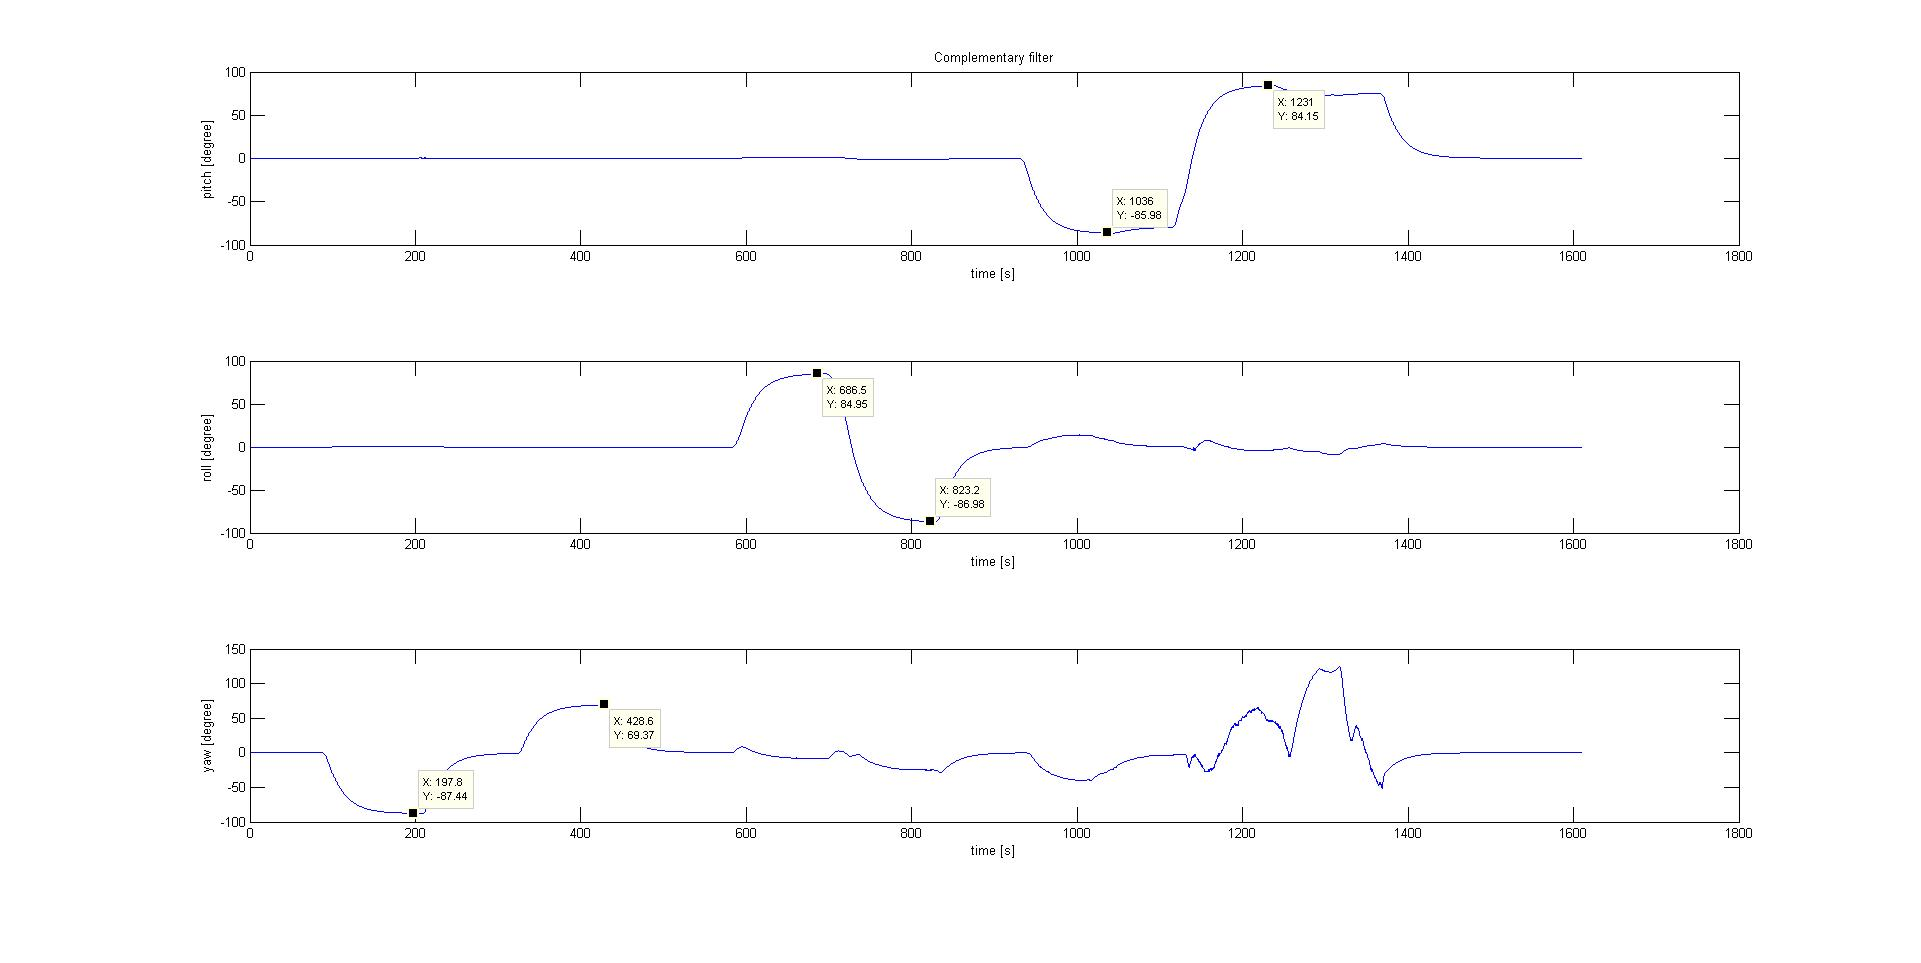
\includegraphics[width=1.0\textwidth]{fig/Res_Kal_Comp/initial_Comp}
	\caption{First result complementary filter}
	\label{fig:initial_Comp}
\end{figure}

First what catches somebody's eye is that the filter is to slow. So the steady state value is achieved after consuming to much time. Also the yaw angle is not equally distributed over the whole 360 degree. In one direction the angle changes just around 70 degree. When changing roll the influences in yaw is just because the rotation was not straight in roll direction. Changing the pitch angle to much lead to a change in yaw. The next step is to improve the yaw angle, so that it will reach also the +90 degree. Also the yaw change during pitch will be observed and compared to the initial measurement. Also the time constant will be changed that a faster response can be seen.
\begin{figure}[H]
	\centering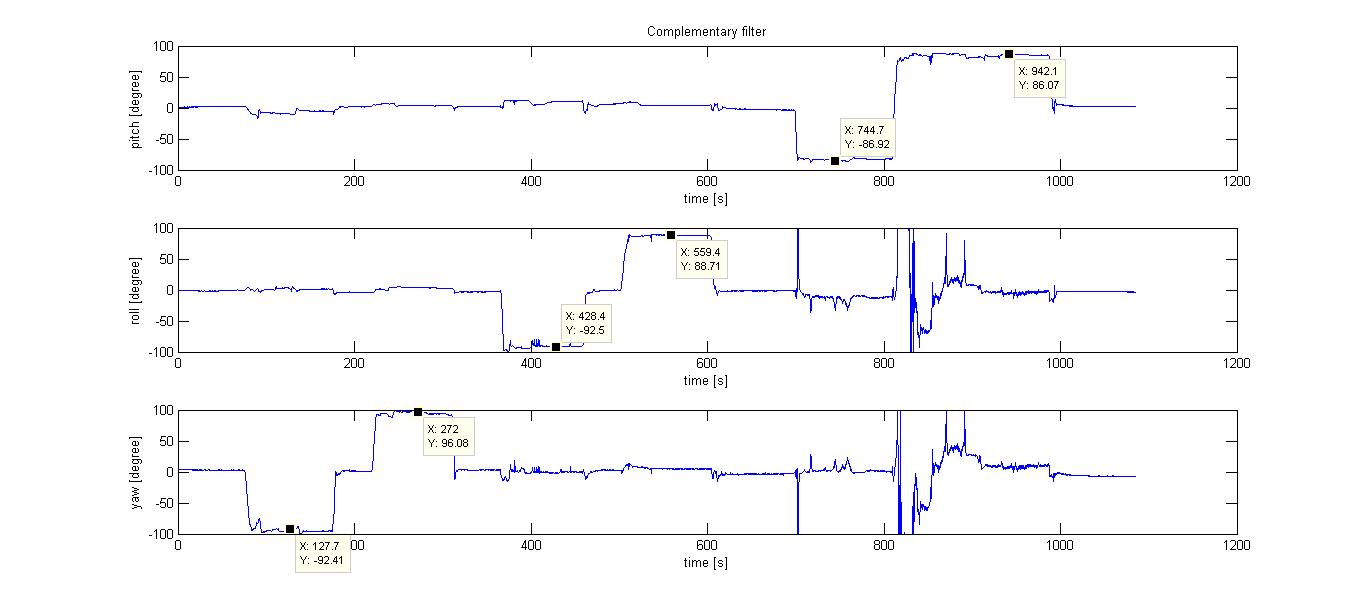
\includegraphics[width=1.0\textwidth]{fig/Res_Kal_Comp/final_Comp1}
	\caption{Final result complementary filter}
	\label{fig:final_Comp}
\end{figure}
The comparison of the first result and the final result shows the increased filter speed. The signal needs not so much time to reach the final value. Also the yaw angle reaches the 90 degree when turning 90 degree. The extreme influences on yaw directly after changing of the rotation angle results from a hand made rotation. The influences on yaw while an other angle is applied is extremely reduced.\\

The last figure shows how off an angle can be when just an gyroscope is used. On the left side the integrated gyroscope can be seen. On the right side, the 3D representation of the fusioned sensors are displayed.
\begin{figure}[H]
	\centering\includegraphics[width=0.6\textwidth]{fig/Res_Kal_Comp/3D}
	\caption[3D representation of Complementary-filtered IMU-Data in MATLAB]{3D representation of the integrated gyroscope raw values on the left and the fusion filtered on the right}
	\label{fig:3D}
\end{figure}

%--------------------------------------------
% section: Kalman Filter result
%--------------------------------------------

\section{Kalman-Filter}
\label{sec:KalmanFilterResult}

For the Kalman filter the noise of the measurement and the process has to be set up. This noise values are the variances of the used sensors and of the process. In the calculation process are those matrices named $\underline Q$ and $\underline R$. The matrix $\underline Q$ uses the variances of the process noise and the matrix $\underline R$ uses the variances of the noise of the sensors.\\\\
\underline{Prediction step:}\\\\
Predict the next state:
\begin{align}
\vec x_k = \underline{A}\vec x_{k-1}+\underline{B}\vec u_{k-1}
\label{equ:KalmanFilterResult:Kalman1}
\end{align}
Predict the covariance for the next step:
\begin{align}
\underline{P}_k = \underline{A}\underline{P}_{k-1}\underline{A}^T+\underline{Q}
\label{equ:KalmanFilterResult:Kalman2}
\end{align}
\underline{Correction step:}\\\\
Computation of the Kalman gain:
\begin{align}
\underline{K}_k = \underline{P}_k	\underline{H}^T(\underline{H}\underline{P}_k\underline{H}^T+\underline{R})^{-1}
\label{equ:KalmanFilterResult:Kalman3}
\end{align}
Updating state prediction with new measurement:
\begin{align}
\vec x_k = 	\vec x_k+\underline{K}_k(\vec z_k-\underline{H}\vec x_k)
\label{equ:KalmanFilterResult:Kalman4}
\end{align}
Updating the error covariance:
\begin{align}
\underline{P}_k = (\underline{I}-\underline{K}_k\underline{H})\underline{P}_k	
\label{equ:KalmanFilterResult:Kalman5}
\end{align}
As an initial guess the matrices are set to:
\begin{align}
\underline{Q} &= \begin{pmatrix} 0.005&0&0 \\ 0&0.005&0 \\ 0&0&0.0001 \end{pmatrix}\\
\underline{R} &= \begin{pmatrix} 0.5&0&0 \\ 0&0.5&0 \\ 0&0&0.01 \end{pmatrix}
\end{align}
With those matrices the following result was achieved. To make a test, first the yaw angle is changed in the range of $\pm90 \degree$, after that a roll angle is changed in the range of $\pm90 \degree$ and finally the pitch angle is changed in the range of $\pm90 \degree$. 

\begin{figure}[H]
	\centering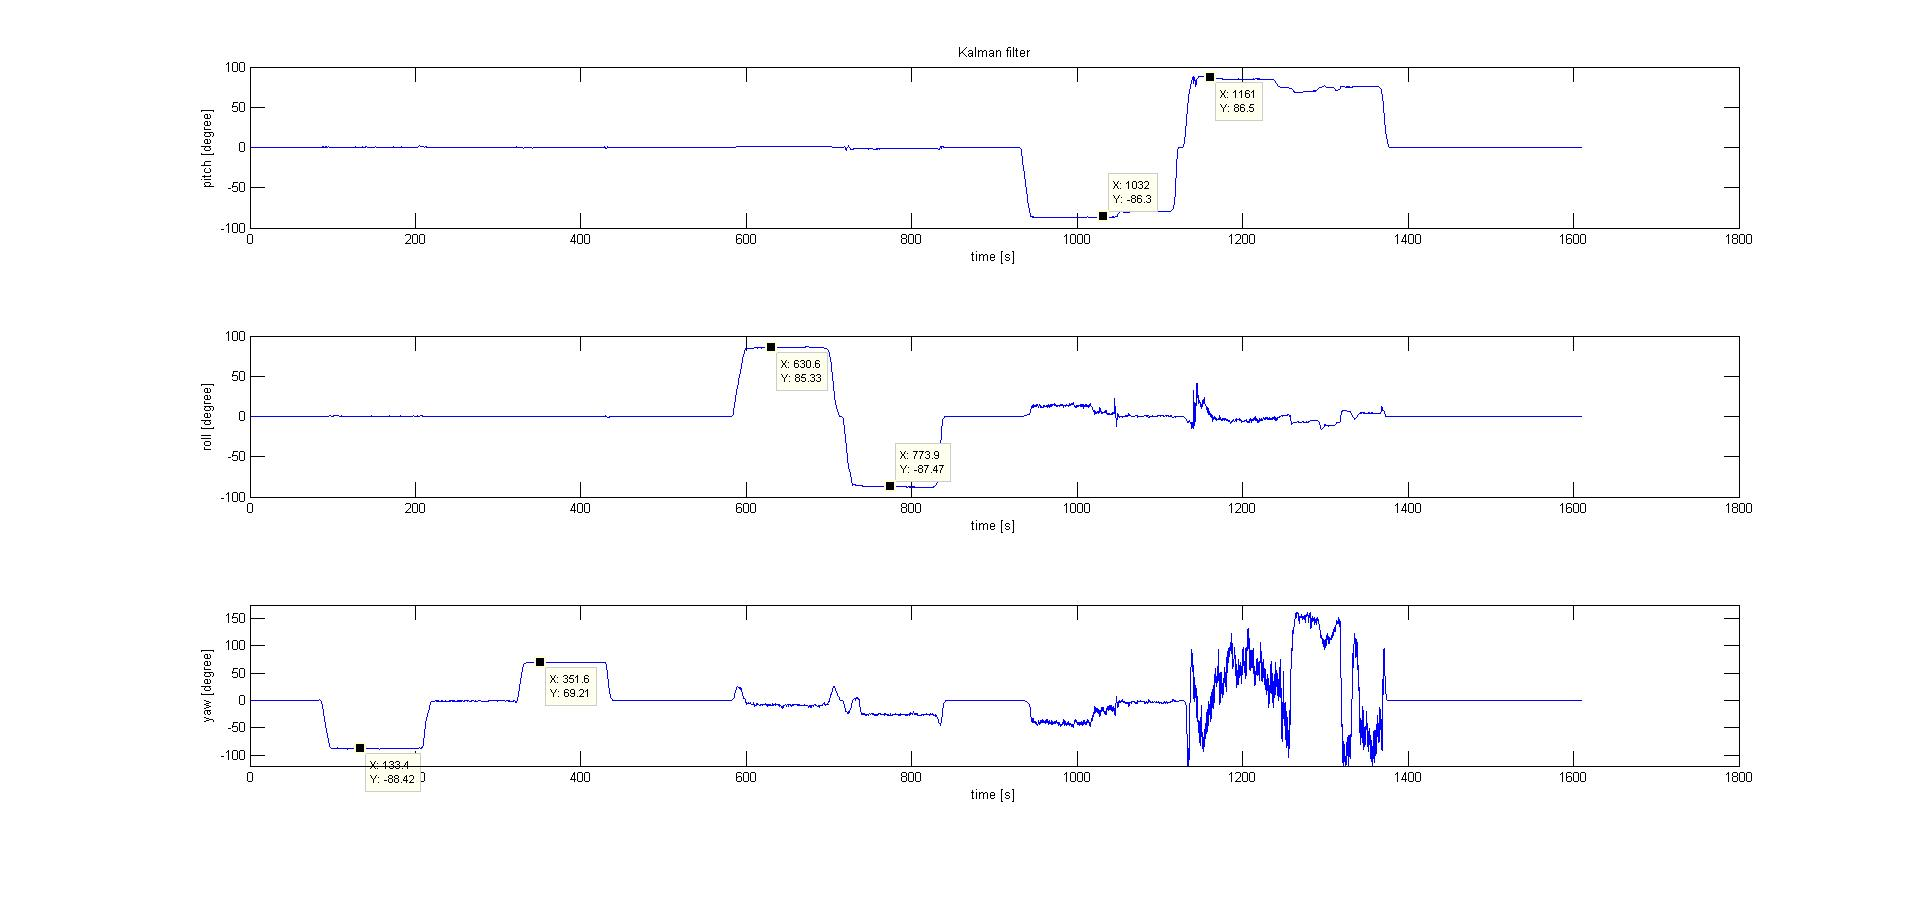
\includegraphics[width=1.0\textwidth]{fig/Res_Kal_Comp/initial_Kalman}
	\caption{First result Kalman filter}
	\label{fig:initial_Kalman}
\end{figure}

The filter responses in a adequate time. Yaw angle change is like with the complementary filter from -90 degree to just 70 degree. The roll angle changes sufficient. But when changing the pitch angle to high a extreme yaw angle change can be seen. So the next step is to improve the yaw angle, so that it will reach also the +90 degree. Also the yaw change during pitch will be observed. After measuring the mean value and variances of all sensors they can be used to improve the Kalman filter. The figures \ref{fig:varAcc}, \ref{fig:varGyro} and \ref{fig:varMag} show the logged data.
\begin{figure}[H]
	\centering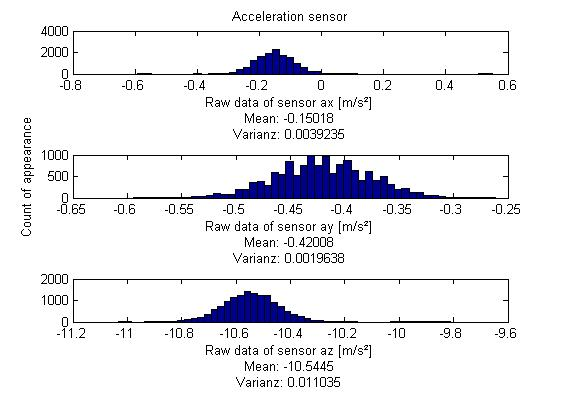
\includegraphics[width=0.8\textwidth]{fig/Res_Kal_Comp/varAcc3}
	\caption{Analyzing the acceleration sensor}
	\label{fig:varAcc}
\end{figure}
\begin{figure}[H]
	\centering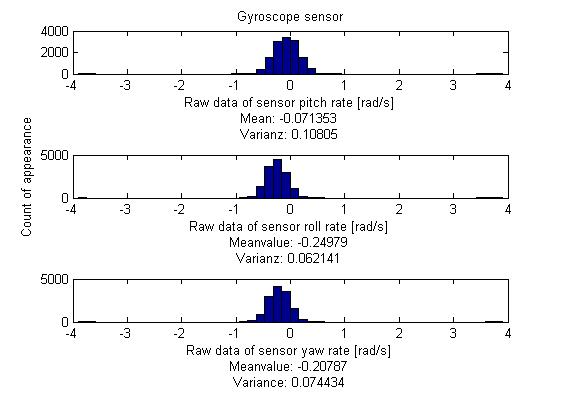
\includegraphics[width=0.8\textwidth]{fig/Res_Kal_Comp/varGyro3}
	\caption{Analyzing the gyroscope sensor}
	\label{fig:varGyro}
\end{figure}
\begin{figure}[H]
	\centering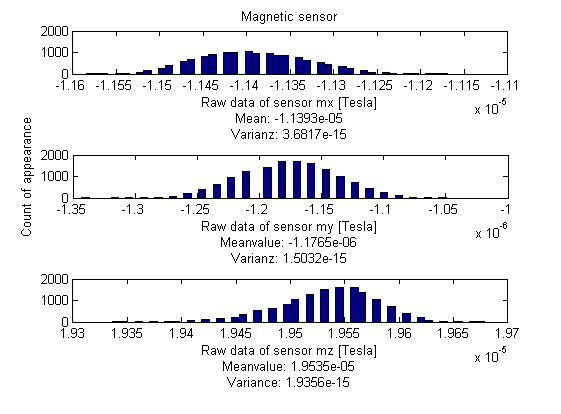
\includegraphics[width=0.8\textwidth]{fig/Res_Kal_Comp/varMag3}
	\caption{Analyzing the magnetic sensor}
	\label{fig:varMag}
\end{figure}
First the matrix $\underline Q$, the variances of the process noise and the matrix $\underline R$, the variances of the measured sensor noises are changed by using the measured values. The new values are:\\
\begin{align}
\underline{Q} &= \begin{pmatrix} 0.005&0&0 \\ 0&0.005&0 \\ 0&0&0.005 \end{pmatrix}\\
\underline{R} &= \begin{pmatrix} 0.06&0&0 \\ 0&0.1&0 \\ 0&0&0.07 \end{pmatrix}
\end{align}

\begin{figure}[H]
	\centering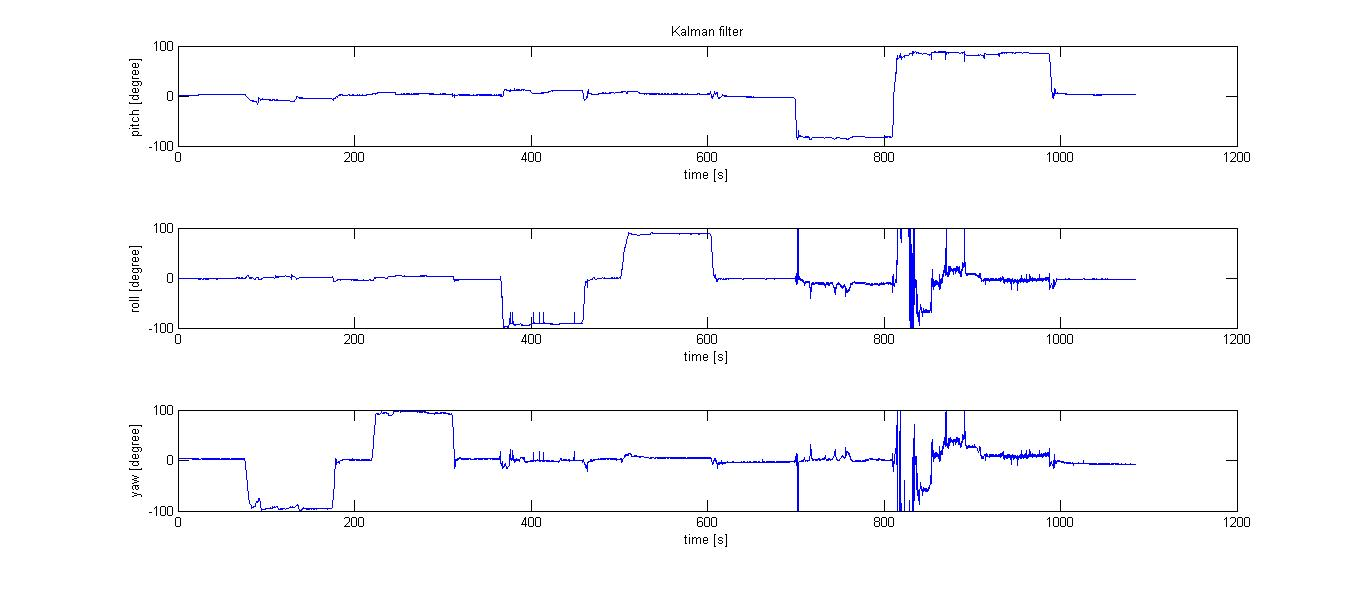
\includegraphics[width=1.0\textwidth]{fig/Res_Kal_Comp/final_Kalman1}
	\caption{Final result Kalman filter}
	\label{fig:final_Kalman}
\end{figure}
The wanted improving of the yaw angle in reaching the 90 degree when turning 90 degree is successfully reached. The extreme influences on yaw directly after changing of the rotation angle results from a hand made rotation. The influences on yaw while an other angle is applied is extremely reduced.\\

The last figure shows how off an angle can be when just an gyroscope is used. On the left side the integrated gyroscope can be seen. On the right side, the 3D representation of the fusioned sensors are displayed.
\begin{figure}[H]
	\centering\includegraphics[width=0.6\textwidth]{fig/Res_Kal_Comp/3D}
	\caption[3D representation of Kalman-filtered IMU-Data in MATLAB]{3D representation of the integrated gyroscope raw values on the left and the fusion filtered on the right}
	\label{fig:KalmanFilterResult:3D}
\end{figure}

%--------------------------------------------
% section: Complementary Filter description
%--------------------------------------------
\newpage
\section{Sensor fusion for Inertial Measurement Unit}
\label{sec:Sensor fusion for Inertial Measurement Unit}


For enabling a autonomous flight, the Raspberry Pi has to know the orientation. Figure \ref{fig:angles} shows the axes and the naming of the rotation around the axes. These rotations are later used for the calculation for the roll, pitch and yaw angles.

\begin{figure}[H]
	\centering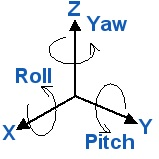
\includegraphics[width=0.3\textwidth]{fig/Kal_Comp/Roll_pitch_yaw}
	\caption{Roll, Pitch, Yaw \cite{doc:boreg}}
	\label{fig:angles}
\end{figure}

To get reliable and stable orientation of the Raspberry Pi and so from the Quadrocopter several sensors can be used. Either a acceleration sensor, a magnetic sensor or a gyroscope can be used. But each of them have some drawbacks.\\
The acceleration sensor is very fast and delivers reliable pitch and roll angles, but the yaw angle itself can't be calculated. Another problem is, that due to vibrations a smooth angle is not possible to calculate.\\\\
The magnetometer can be used to calculate the heading, this means the yaw angle but not the roll and pitch angle. Another problem when the sensor has a roll and pitch angle, the heading can not be easily calculated. In this case a tilt compensation has to be done. In the figure \ref{fig:Mag_Acc} the logging of the pitch and roll angle calculated from the acceleration sensor and the yaw angle calculated with the magnetometer can be seen. When those sensors are not combined errors occur during the calculation. In the time from 250 seconds to 450 seconds a yaw angle is applied which leads just to a yaw angle change. In the time area from 500 seconds to 600 seconds a roll angle is applied which also leads to a yaw change which is an error. In the time area from 700 seconds to 800 seconds a pitch angle is applied which also leads to a yaw change which is an error.\\

When designing a system using multiple MEMS sensors, it is important to understand the advantages and disadvantages of accelerometers, gyroscopes, magnetometers, and pressure sensors.

Sensor fusion solves key motion sensing performance issues of 6-axis modules consisting of a 3-axis accelerometer and a 3-axis gyroscope or a 3-axis accelerometer and a 3-axis magnetic sensor. 1) A 6-axis inertial module with an accelerometer and a gyroscope loses its absolute orientation as the gyro drifts over time, requiring calibration to restore accurate heading reference. 2) A 6-axis module with accelerometer and magnetometer is prone to data corruption in the presence of ferrous materials in the environment. 3) A 9-axis module with an accelerometer, a gyroscope and a magnetometer eliminates the drift that occurs with stand-alone sensor solutions. But these can be subject to magnetic interference. Algorithms to fuse the sensor data are required to compensate for the magnetic interference.

\begin{figure}[H]
	\centering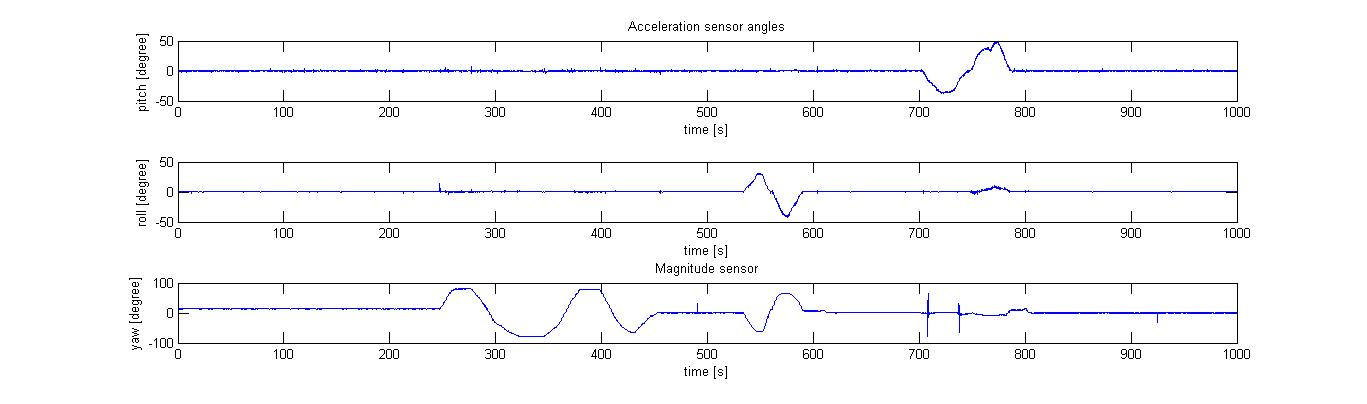
\includegraphics[width=1.0\textwidth]{fig/Kal_Comp/Magn_Acc.jpg}
	\caption{Magnetic / Acceleration angles}
	\label{fig:Mag_Acc}
\end{figure}

The last sensor is the gyroscope. The angle can be easily calculated by integrating the rates of the gyroscope. The sensor is not as fast as the acceleration sensor. So vibrations make no problems for the calculation. But due to the problem of the offset of the gyroscope, the angles will be drifting because of the integration of the rotation rates. This can be seen in figure \ref{fig:Comp_gyro}\\\\

\begin{figure}[H]
	\centering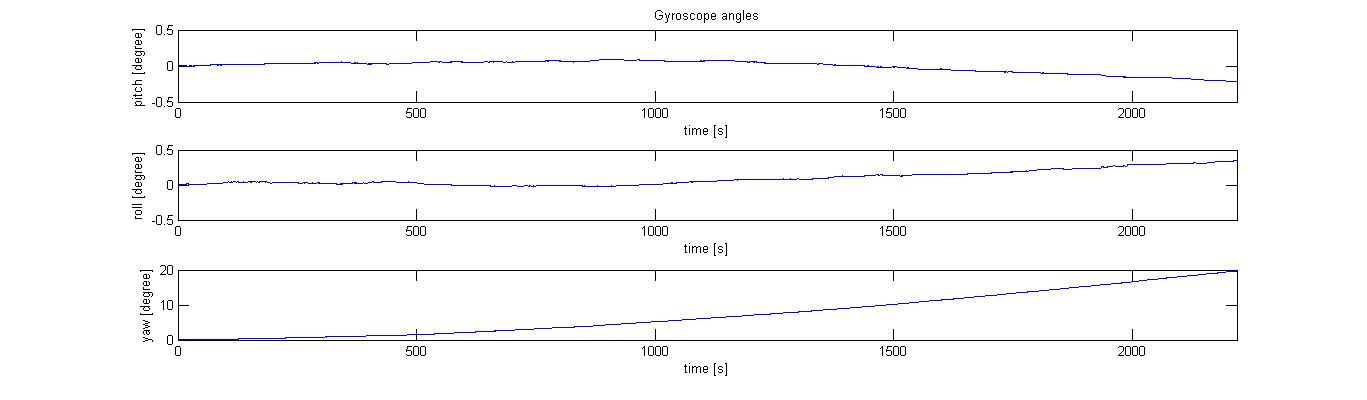
\includegraphics[width=1.0\textwidth]{fig/Kal_Comp/Comp_gyro.jpg}
	\caption{Gyroscope angles}
	\label{fig:Comp_gyro}
\end{figure}

To use all positive features of the sensors and reduce the negative drawbacks a sensor fusion is the needed solution. There are many possibilities for fusion algorithms. In this project a Complementary-Filter and Kalman-Filter is implemented.

%--------------------------------------------
% section: Complementary Filter description
%--------------------------------------------
\newpage
\section{Complementary-Filter}
\label{sec:ComplementaryFilter}

The first approach for a sensor fusion is the complementary filter. This filter uses a highpass filter for the gyroscopes and a lowpass filter for the acceleration sensor. The highpass filter is used after the integration of the rotation rates. This can be seen in figure \ref{fig:complementary}.\\
\begin{figure}[H]
	\centering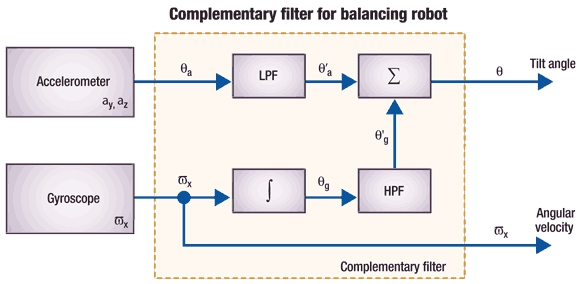
\includegraphics[width=1\textwidth]{fig/Kal_Comp/Complementary.jpg}
	\caption{Complementary-Filter\cite{doc:STM}}
	\label{fig:complementary}
\end{figure}
The implementation effort is extremely lower than with the Kalman Filter. Because here no matrices and matrix operations are needed. Also are there less calculations and so fits this algorithm better to microprocessors. The only thing what needs to be checked is the lowpass/highpass-filter coefficient. Next the needed calculations are mentioned to show the difference of the complementary and Kalman filter.
\begin{itemize}
	\item Calculation of the accelerometer and magnetometer angles
	\item Calculation of the gyroscope angles
	\item Complementary-Filter usage with defined filter time of the lowpass and highpass-filter
\end{itemize}


%--------------------------------------------
% section: Kalman Filter description
%--------------------------------------------
\newpage
\section{Kalman-Filter}
\label{sec:KalmanFilter}

The second approach for a sensor fusion is the Kalman filter. This filter is based on the state space modeling where between the dynamics of the system and the process of the measurement is differentiated. Although the measuring is faulty and the system state is noisy, this filter guesses with the help of a set of equations the correct true state of the system. Instead of using the absolute value it uses the mean value and variance of the normal distribution. The mean value is the perfect measurement and the variance tells the uncertainty of the measurement. Figure \ref{fig:measurement} shows a measurement of an acceleration sensor.
\begin{figure}[H]
	\centering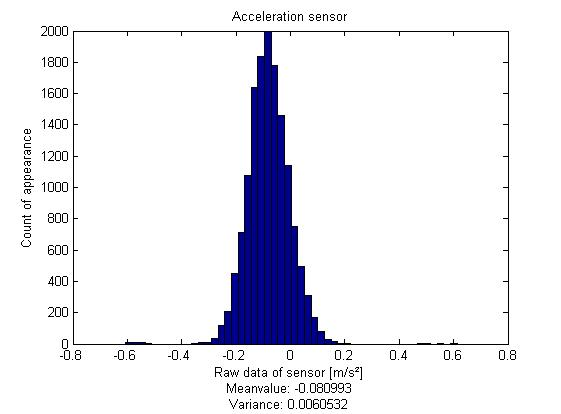
\includegraphics[width=0.8\textwidth]{fig/Kal_Comp/AccX.jpg}
	\caption{Variance and Meanvalue of an acceleration sensor}
	\label{fig:measurement}
\end{figure}

The following state space description shows the calculation of the new states which in the case of this project represent the angles pitch, roll and yaw. Equation \ref{equ:states} shows the defined state vector.
\begin{align}
\vec x = \begin{pmatrix} pitch \\ roll \\ yaw \end{pmatrix}
\label{equ:states}
\end{align}
The calculation of a new state and the output can be seen in the formulas \ref{equ:KalmanModell1} and \ref{equ:KalmanModell2}.
\begin{align}
\vec{x_k} = \underline{A}\vec x_{k-1}+\underline{B}\vec u_{k-1} + W_{k-1}
\label{equ:KalmanModell1}
\end{align}
\begin{align}
\vec y_k = \underline{H}\vec x_k+ V_k
\label{equ:KalmanModell2}
\end{align}
Legend of the formula shown above:\\
\begin{itemize}
	\item $\vec{x}_k$ state vector of actual step
	\item $\vec{x}_{k-1}$ state vector of previous step
	\item $\underline{A}$ system matrix
	\item $\underline{B}$ input matrix
	\item $\vec{u}_{k-1}$ input vector of previous step
	\item $\underline{W}$ process noise
	\item $\vec{y}_{k}$ output vector
	\item $\underline{H}_k$ output matrix
	\item $\underline{V}$ measurement noise
\end{itemize}
Because of the measurement and the process noise the new state is not good. The Kalman filter takes the process and measurement noise into account to improve the state estimation. To do so the Kalman filter is split into two parts, the prediction step (time update) and correction step (measurement update). In the prediction step the filter estimates the states in the next step and calculates the new covariance. Those values are calculated for the states which in the following step are expected to be reached. In the next step, the correction update, the filter checks if the pre-calculated state is reached. According to the difference the correction for the following prediction is done.\\\\
\underline{Prediction step:}\\\\
Predict the next state:
\begin{align}
\vec x_k = \underline{A}\vec x_{k-1}+\underline{B}\vec u_{k-1}
\label{equ:Kalman1}
\end{align}
Predict the covariance for the next step:
\begin{align}
\underline{P}_k = \underline{A}\underline{P}_{k-1}\underline{A}^T+\underline{Q}
\label{equ:Kalman2}
\end{align}

\underline{Correction step:}\\\\
Computation of the Kalman gain:
\begin{align}
\underline{K}_k = \underline{P}_k	\underline{H}^T(\underline{H}\underline{P}_k\underline{H}^T+\underline{R})^{-1}
\label{equ:Kalman3}
\end{align}
Updating state prediction with new measurement:
\begin{align}
\vec x_k = 	\vec x_k+\underline{K}_k(\vec z_k-\underline{H}\vec x_k)
\label{equ:Kalman4}
\end{align}
Updating the error covariance:
\begin{align}
\underline{P}_k = (\underline{I}-\underline{K}_k\underline{H})\underline{P}_k	
\label{equ:Kalman5}
\end{align}
These steps have to be done more than just ones, so when the correction is finished, the update has to be called again and so on.\\
As can be seen the implementation effort is higher than with the Complementary Filter. Because matrices and matrix operations are needed, more calculation steps are needed and the functionality of the Kalman filter is not as intuitive like with the complementary filter. Also the uncertainty of the process itself and the measurement error needs to be known. Nevertheless the results from the Kalman filter are better than those of the complementary filter. This can be seen in the results showing chapter of this project.

%--------------------------------------------
% section: Matrix Lib
%--------------------------------------------
\section{Matrix library}
\label{sec:MatrixLib}

Like already mentioned in the Kalman chapter various matrix operations are needed. So the simple assignment from a matrix to another, the addition and subtraction of a matrix from another. Additionally the multiplication of two matrices, the initialization of a matrix and building of the identity matrix. Finally the transpose of a matrix and the inversion of a matrix.\\
\underline{Assignment:}
\begin{align}		
\underline A&=\underline B\\
A(0,0)&=B(0,0)\\
...\\
A(n,m)&=B(n,m)
\end{align}
\underline{Addition/Subtraction:}
\begin{align}		
\underline A&=\underline B \pm \underline C\\
A(0,0)&=B(0,0)\pm C(0,0)\\
...\\
A(n,m)&=B(n,m)\pm C(n,m)
\end{align}
\underline{Multiplication:}
\begin{align}		
\underline A&=\underline B \cdot \underline C\\
A(0,0)&=B(0,0)\cdot C(0,0)+...+B(0,m)\cdot C(n,0)\\
...\\
A(n,m)&=B(n,0)\cdot C(0,m)+...+B(n,m)\cdot C(n,m)
\end{align}
\underline{Initialization:}
\begin{align}		
A(0,0)&=xx.xx\\
A(0,1)&=xx.xx\\
...\\
A(1,0)&=xx.xx\\
...\\
A(n,m)&=xx.xx
\end{align}
\underline{Identity matrix:}
\begin{align}		
A(0,0)&=1\\
A(0,1)&=0\\
...\\
A(1,0)&=0\\
A(1,1)&=1\\
...\\
A(n,n)&=1
\end{align}
\underline{Transpose a matrix:}
\begin{align}		
A(0,0)&=A(0,0)\\
A(0,1)&=A(1,0)\\
...\\
A(3,0)&=A(0,3)\\
A(4,0)&=A(0,4)\\
...\\
A(n,n)&=A(n,n)
\end{align}
\underline{Invert a matrix:}\\
To ensure that the inversion not only works with small matrices, the implementation uses a different way. So first the Cholesky method is used to build a lower triangular matrix. Next step is solving a linear system to get the inverse of the matrix. With this method all sizes of matrices can be inverted. It just has to be positive definite.

%--------------------------------------------
% section: Sensor fusion controlling
%--------------------------------------------
\newpage
\section{Sensor fusion controlling}
\label{sec:SensFusContr}

To obtain the statistical data of all sensors of the inertial measurement unit a Matlab model is used. This model also helps to check the results of the two different fusion filters, the Kalman filter and the complementary filter. The data is send via UDP-packets from the Raspberry Pi to the Matlab model on the Host computer. Figure \ref{fig:model} shows the used Matlab model. Additional a 3D representation of the rotations is visualized and can be directly compared with the integrated offset corrected gyroscope data.

\begin{figure}[H]
	\centering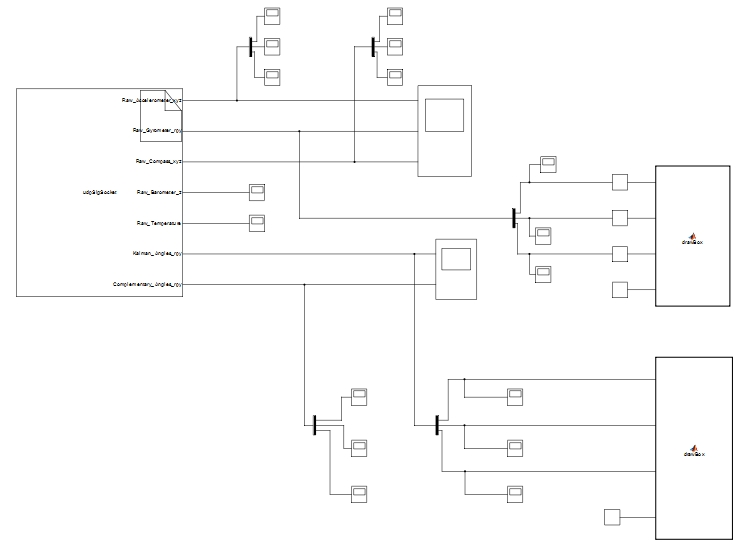
\includegraphics[width=1\textwidth]{fig/Res_Kal_Comp/Model}
	\caption{Matlab model}
	\label{fig:model}
\end{figure}

\newpage
With the help of the scopes within this model, the logged data is stored in the Matlab workspace and then it is analyzed with a Matlab file. With the help of this file, a histogram from every sensor is generated. Also the mean value and the variance from those sensor is calculated. Finally a plot from the complementary filter and Kalman filter is generated. Also the needed minimum and maximum values of the magnetic sensor is stored. This needs to be done to reduce the influences of hard magnetic parts to the magnetic sensor. Those stored minimum and maximum values are then written in a header file (OrientationDefines.h) which needs to be copied to the folder of the Orientation.c and Orientation.h files. To achieve the best performance, the description of chapter \ref{sec:angle} needs to be followed.

%\lstset{language=Matlab,%
%backgroundcolor=\color{white}  
%}

\begin{lstlisting}[caption={[MATLAB script to calibrate the magnetometer]MATLAB script to calibrate the magnetometer and automatically generate a header file with calibration data.}, label=code:SensFusContr:calibMagMatlab,language=MATLAB]
headerFileName = 'OrientationDefines.h';

%Acceleration sensor
figure(1)
%plot histogram of ax and calculate meanvalue and variance
subplot(3,1,1)
hist(ax.signals.values(:),50);
    M=mean(ax.signals.values(:));
    V=var(ax.signals.values(:));
title('Acceleration sensor')
disp(['Meanvalue: ' num2str(M)])
xlabel({'Raw data of sensor ax' ['Mean: ' num2str(M)] ['Varianz: ' num2str(V)]}) % x-axis label

%plot histogram of ay and calculate meanvalue and variance
subplot(3,1,2)
hist(ay.signals.values(:),50);
    M=mean(ay.signals.values(:));
    V=var(ay.signals.values(:));
xlabel({'Raw data of sensor ay' ['Mean: ' num2str(M)] ['Varianz: ' num2str(V)]}) % x-axis label
ylabel('Count of appearance') % y-axis label

%plot histogram of az and calculate meanvalue and variance
subplot(3,1,3)
hist(az.signals.values(:),50);
    M=mean(az.signals.values(:));
    V=var(az.signals.values(:));
xlabel({'Raw data of sensor az' ['Mean: ' num2str(M)] ['Varianz: ' num2str(V)]}) % x-axis label

%Magnetic sensor
figure(2)
%plot histogram of mx and calculate meanvalue and variance
subplot(3,1,1)
hist(mx.signals.values(:),50);
    M=mean(mx.signals.values(:));
    V=var(mx.signals.values(:));
title('Magnetic sensor')
disp(['Meanvalue: ' num2str(M)])
xlabel({'Raw data of sensor mx' ['Mean: ' num2str(M)] ['Varianz: ' num2str(V)]}) % x-axis label

%plot histogram of my and calculate meanvalue and variance
subplot(3,1,2)
hist(my.signals.values(:),50);
    M=mean(my.signals.values(:));
    V=var(my.signals.values(:));
xlabel({'Raw data of sensor my' ['Meanvalue: ' num2str(M)] ['Varianz: ' num2str(V)]}) % x-axis label
ylabel('Count of appearance') % y-axis label

%plot histogram of mz and calculate meanvalue and variance
subplot(3,1,3)
hist(mz.signals.values(:),50);
    M=mean(mz.signals.values(:));
    V=var(mz.signals.values(:));
xlabel({'Raw data of sensor mz' ['Meanvalue: ' num2str(M)] ['Variance: ' num2str(V)]}) % x-axis label

%Gyroscope sensor
figure(3)
%plot histogram of pitch and calculate meanvalue and variance
subplot(3,1,1)
hist(pitch.signals.values(:),50);
    M=mean(pitch.signals.values(:));
    V=var(pitch.signals.values(:));
title('Gyroscope sensor')
disp(['Meanvalue: ' num2str(M)])
xlabel({'Raw data of sensor pitch rate' ['Mean: ' num2str(M)] ['Varianz: ' num2str(V)]}) % x-axis label

%plot histogram of roll and calculate meanvalue and variance
subplot(3,1,2)
hist(roll.signals.values(:),50);
    M=mean(roll.signals.values(:));
    V=var(roll.signals.values(:));
xlabel({'Raw data of sensor roll rate' ['Meanvalue: ' num2str(M)] ['Varianz: ' num2str(V)]}) % x-axis label
ylabel('Count of appearance') % y-axis label

%plot histogram of yaw and calculate meanvalue and variance
subplot(3,1,3)
hist(yaw.signals.values(:),50);
    M=mean(yaw.signals.values(:));
    V=var(yaw.signals.values(:));
xlabel({'Raw data of sensor yaw rate' ['Meanvalue: ' num2str(M)] ['Variance: ' num2str(V)]}) % x-axis label


%Complementary filter
figure(4)
subplot(3,1,1)
plot(Comp_pitch.time,Comp_pitch.signals.values(:));
title('Complementary filter')
xlabel('time [s]') % x-axis label
ylabel('pitch [degree]') % y-axis label

subplot(3,1,2)
plot(Comp_roll.time,Comp_roll.signals.values(:));
xlabel('time [s]') % x-axis label
ylabel('roll [degree]') % y-axis label

subplot(3,1,3)
plot(Comp_yaw.time,Comp_yaw.signals.values(:));
xlabel('time [s]') % x-axis label
ylabel('yaw [degree]') % y-axis label


%Kalman filter
figure(5)
subplot(3,1,1)
plot(Kalman_pitch.time,Kalman_pitch.signals.values(:));
title('Kalman filter')
xlabel('time [s]') % x-axis label
ylabel('pitch [degree]') % y-axis label

subplot(3,1,2)
plot(Kalman_roll.time,Kalman_roll.signals.values(:));
xlabel('time [s]') % x-axis label
ylabel('roll [degree]') % y-axis label

subplot(3,1,3)
plot(Kalman_yaw.time,Kalman_yaw.signals.values(:));
xlabel('time [s]') % x-axis label
ylabel('yaw [degree]') % y-axis label

%min max of magnetic sensor
maxz=max(mz.signals.values)*1000000;
minz=min(mz.signals.values)*1000000;
maxy=max(my.signals.values)*1000000;
miny=min(my.signals.values)*1000000;
maxx=max(mx.signals.values)*1000000;
minx=min(mx.signals.values)*1000000;

fprintf('\n');
disp('Calibration Data:');
disp('=================');
disp(['Min_X: ' num2str(minx)])
disp(['Max_X: ' num2str(maxx)])
disp(['Min_Y: ' num2str(miny)])
disp(['Max_Y: ' num2str(maxy)])
disp(['Min_Z: ' num2str(minz)])
disp(['Max_Z: ' num2str(maxz)])
fprintf('\n');

disp('==================================');
disp('Generating Calibration-Header-File');
disp('==================================');

disp(['Writing header ', headerFileName, ' ...' ]);
fileID = fopen(headerFileName,'w');
fprintf(fileID,'/*!\n');
fprintf(fileID,' * \\file OrientationDefines.h\n');
fprintf(fileID,' */\n');
fprintf(fileID,'\n');
fprintf(fileID,'#ifndef SIG_ORIENTATION_ORIENTATIONDEFINES_H_\n');
fprintf(fileID,'#define SIG_ORIENTATION_ORIENTATIONDEFINES_H_\n');
fprintf(fileID,'\n');
fprintf(fileID,'//Defines for Acceleration Magnetic angle calculation (automatic calibration via MATLAB)\n');
fprintf(fileID,'#define M_SIGORI_MAG_MINX_F64	%.9f\n',minx);
fprintf(fileID,'#define M_SIGORI_MAG_MAXX_F64	%.9f\n',maxx);
fprintf(fileID,'#define M_SIGORI_MAG_MINY_F64	%.9f\n',miny);
fprintf(fileID,'#define M_SIGORI_MAG_MAXY_F64	%.9f\n',maxy);
fprintf(fileID,'#define M_SIGORI_MAG_MINZ_F64	%.9f\n',minz);
fprintf(fileID,'#define M_SIGORI_MAG_MAXZ_F64	%.9f\n',maxz);
fprintf(fileID,'\n');
fprintf(fileID,'#endif /* SIG_ORIENTATION_ORIENTATIONDEFINES_H_ */\n');
fclose(fileID);
disp('Done');
fprintf('\n');
disp('Calibration successfully processed.');

\end{lstlisting}



